%% ------------------------------------------------------------------------- %%
\chapter{Conceitos}
\label{cap:conceitos}

Este capítulo apresenta, um a um, os conceitos mais elementares, 
e tenta harmonizar a terminologia empregada no decorrer do texto.


%% ------------------------------------------------------------------------- %%
\section{\Gls{tectonic}}
\index{\gls{tectonic}}
\label{sec:02_tectonica}

A \gls{tectonic} é \glsdesc*{tectonic}.

Uma das principais evidências das transformações geológicas do planeta 
são os \glspl{equake}. A figura \ref{f:global_epicenters} \citep{img_world_epicenters}
é um mapa global com a ocorrência geográfica dos tremores. Nele é possivel notar que 
os sismos não são distribuídos uniformemente pelo globo.

\begin{figure}[H]
   \centering
   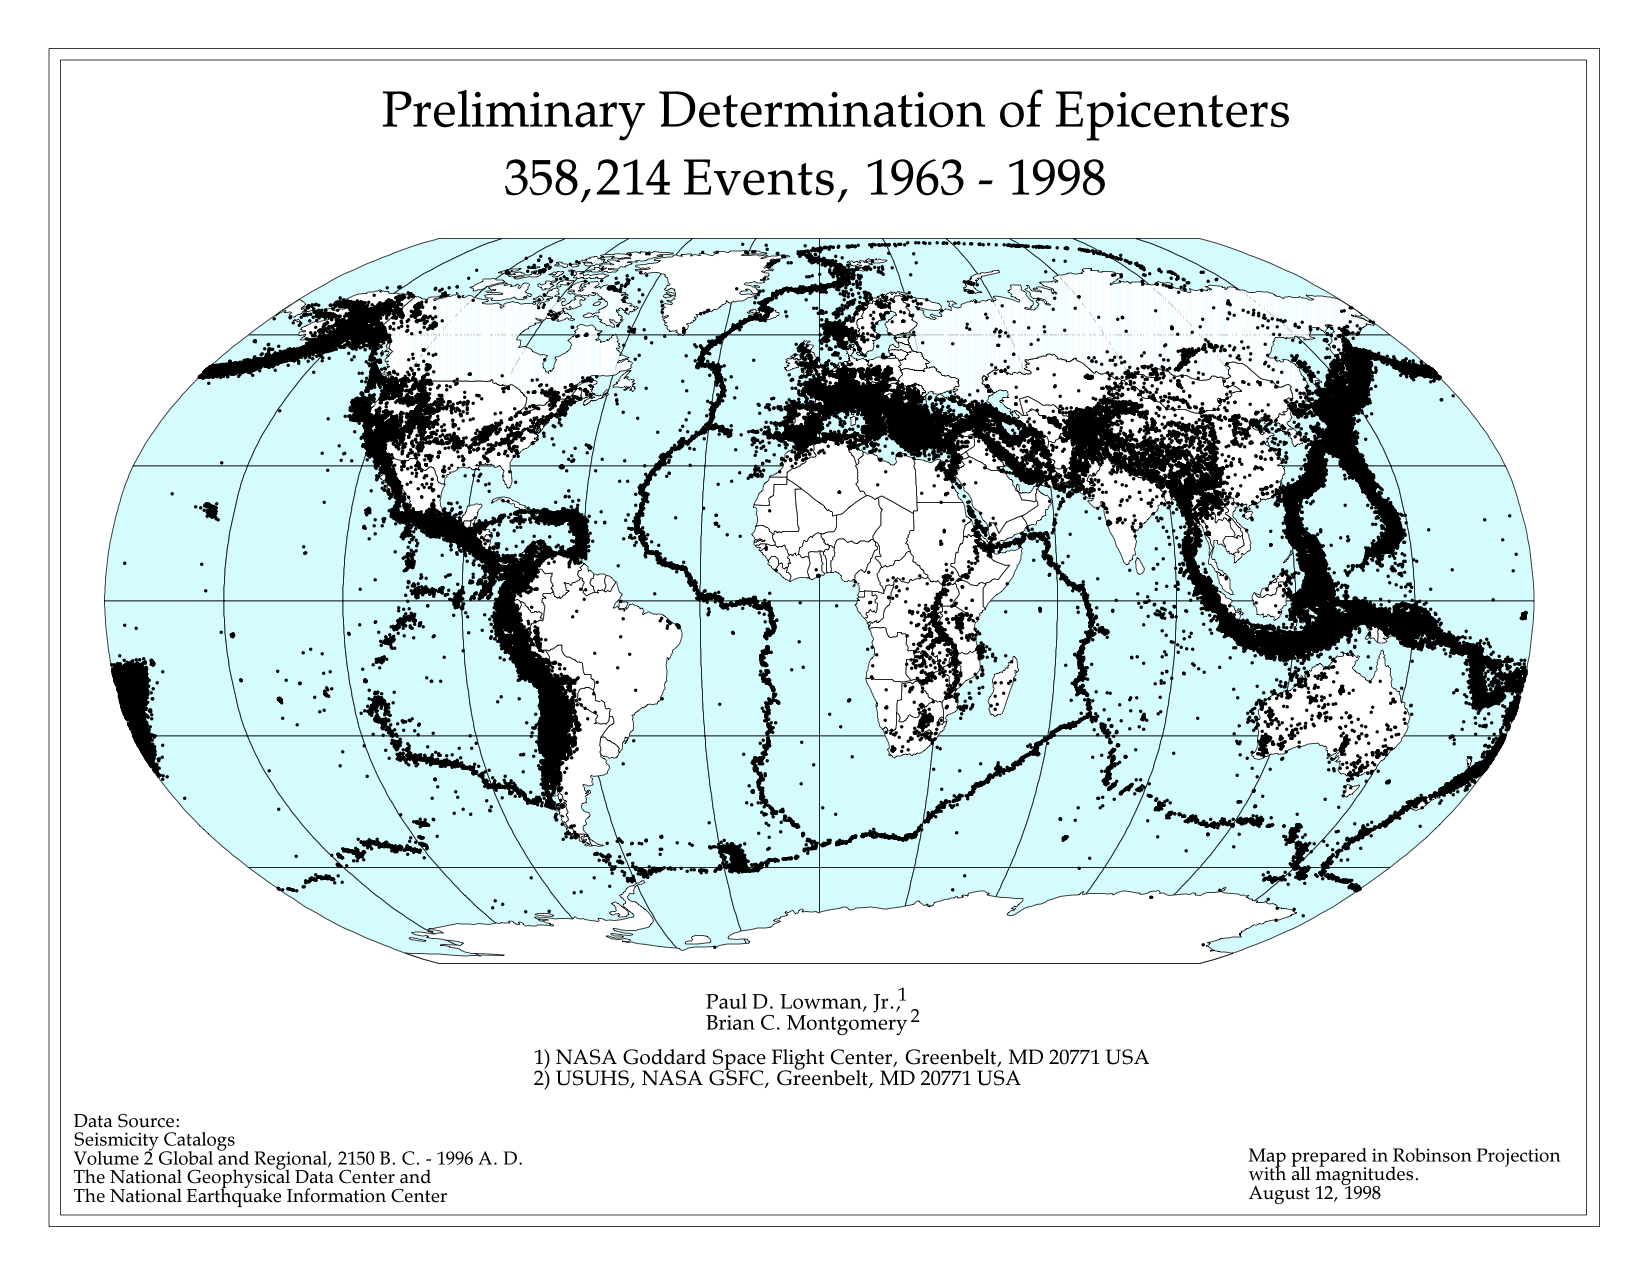
\includegraphics[width=0.80\textwidth]{global_pde_mag_all}
   \caption[Mapa Mundial de Epicentros 1963-1998]
   		   {Mapa Mundial de Epicentros 1963-1998\footnotemark} 
   \label{f:global_epicenters}
\end{figure} 
\footnotetext{\citet{img_world_epicenters}}
 
O padrão apresentado pela \gls{seismic_activity} global foi essencial 
para o desenvolvimento posterior da \gls*{tectonic_plate_theory}.

%% ------------------------------------------------------------------------- %%
\subsection{\Gls{tectonic_plate_theory}}
\index{\Gls{tectonic}!\Gls{tectonic_plate_theory}}
\label{sec:02_placas}

A \gls*{tectonic_plate_theory}, desenvolvida na segunda metade do século XX,
cartografava na superfície do globo as \glspl{litho_plate}.


\begin{figure}[H]
   \centering
   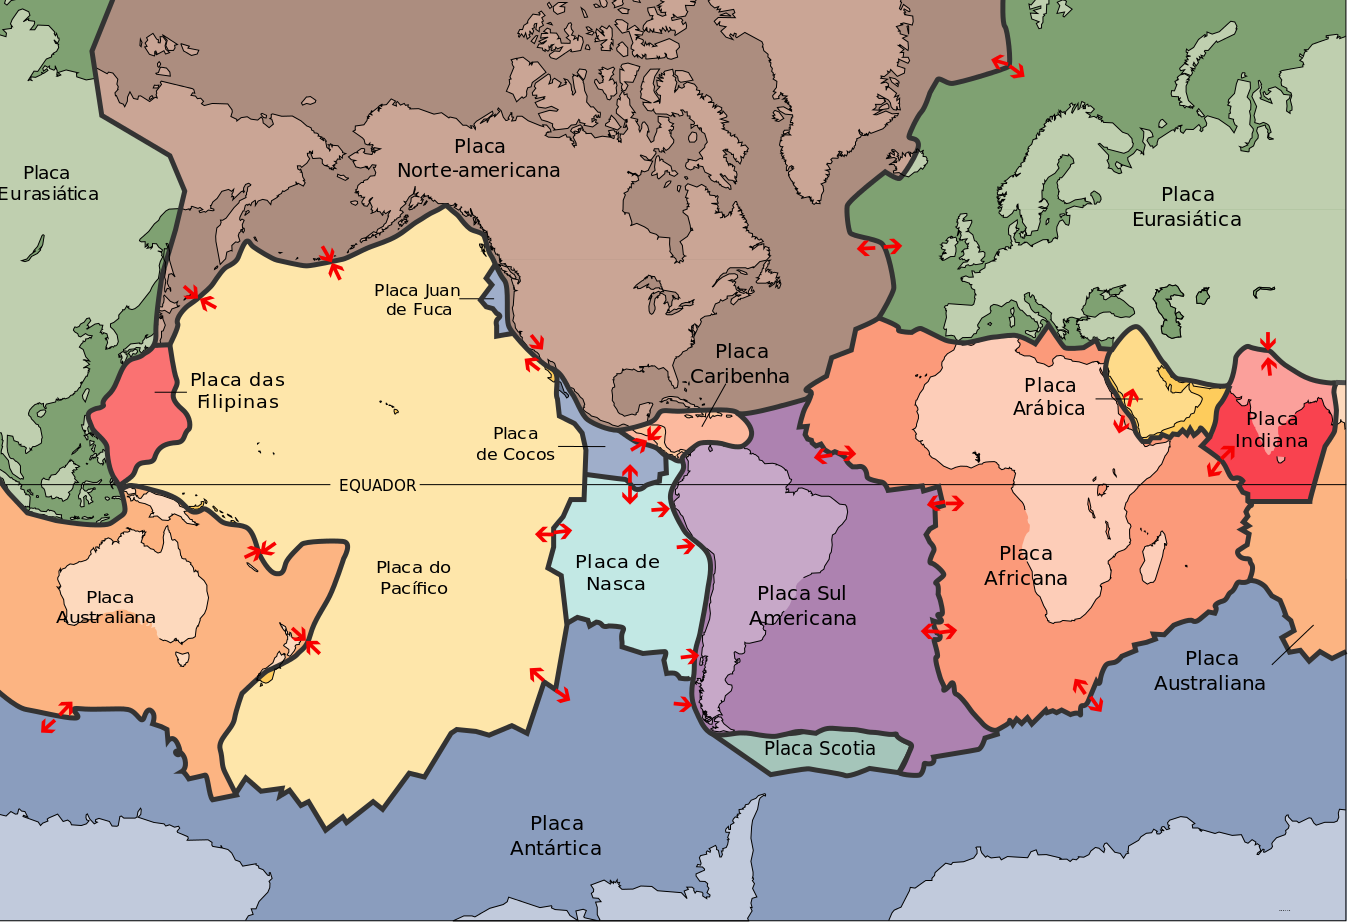
\includegraphics[width=0.80\textwidth]{litho_plates_overview}
   \caption[Cartografia das placas litosféricas]
   		   {Cartografia das placas litosféricas\footnotemark} 
   \label{f:plates_overview}
\end{figure} 
\footnotetext{\citet{img_plates_overview}}
 

As \glspl{litho_plate}, como pode ser visto na figura \ref{f:plates_overview},
e o conceito de \gls{astenosphere} (\glsdesc{astenosphere}) 
surgem para conformar uma teoria capaz de explicar
uma série de fenômenos tectônicos já observados e ainda não bem explicados na época
de seu desenvolvimento. 


%% ------------------------------------------------------------------------- %%
\subsubsection{Bordas}
\index{\Gls{tectonic_plate_theory}!bordas}
\label{sec:02_bordas}

Nas bordas das \glspl{litho_plate}, a tectônica é mais intensa, 
provocando uma enorme diversidade de fenômenos geológicos de acordo
com o tipo de interação, como ilustrado na figura \ref{f:plate_boundaries}.

\begin{figure}[H]
   \centering
   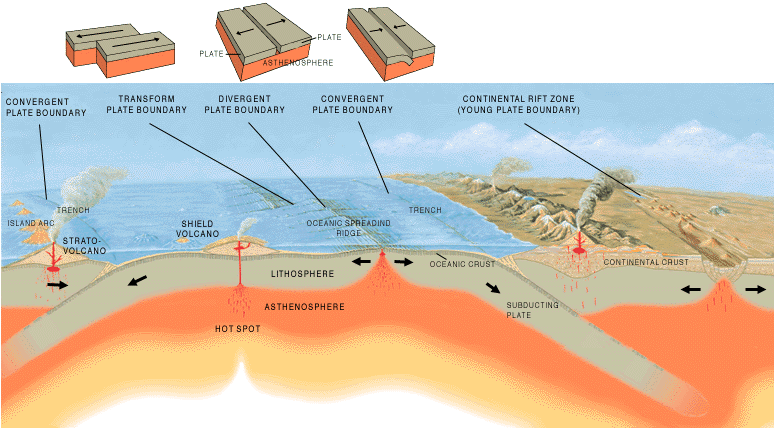
\includegraphics[width=0.80\textwidth]{plate_boundaries}
   \caption[Diferentes tipos de interações entre \glspl{litho_plate} em suas bordas]
   		   {Diferentes tipos de interações entre \glspl{litho_plate} em suas bordas\footnotemark} 
   \label{f:plate_boundaries}
\end{figure} 
\footnotetext{\citet{img_plate_boundaries}}
 
Na figura \ref{f:plate_boundaries} estão ilustrados os diferentes tipos de interação 
entre as \glspl{litho_plate} nas suas bordas, que causam, como já se sabe, a maior
parte dos \glspl{equake} e vulcanismo.

Só na borda das placas é liberada cerca de 95\% da quantidade total da energia 
disseminada na forma de \glspl{equake} no globo.

%% ------------------------------------------------------------------------- %%
\subsubsection{Interior}
\index{\Gls{tectonic_plate_theory}!interior}
\label{sec:02_interior}

A dificuldade maior é explicar, com maior detalhe, porque e como são liberados os outros 
5\% do total de energia em \glspl{equake}, mais raros, no interior das \glspl{litho_plate}.

Não há pleno consenso nem um modelo geral para a explicação do mecanismo de ocorrência dos
sismos no interior das placas, embora sejam conhecidas diversas zonas sísmicas em regiões no interior
de placas, como em Nova Madrid, nos Estados Unidos e também em locais da China e da Austrália para citar alguns.


%% ------------------------------------------------------------------------- %%
\subsection{Sismotectônica}
\index{\gls{tectonic}!\gls{seismotectonic}}
\label{sec:sismotectonica}

A \gls{seismotectonic} é \glsdesc*{seismotectonic}. 

Na prática consiste por um lado, num esforço de compreensão dos
processos geológicos através da observação dos tremores e analogamente, compreender os tremores através da observação
de processos geológicos mensuráveis.  

É fácil notar, portanto, a contribuição dessa disciplina para a análise de sismicidade.







\section{Probabilidade}
\index{probabilidade}
\label{sec:probabilidade}



\subsection{\Glsdesc{pdf}}
\index{\glsdesc{pdf}}
\label{sec:pdf}

A \gls{pdf} é uma função contínua de uma \gls{va}  
que descreve a verossimilhança relativa de que essa \gls{va} 
assuma, entre todas as realizações possíveis, uma em especial.

Considerando, por exemplo, que $f_X(x)$ seja uma \gls{pdf} para a \gls{va} $X$, 
sabe-se que $X$ ocorre como $x$ com probabilidade igual a
\begin{equation}
	P \left\{ X = x\right\} = f_X(x).
	\label{eq:pdf}
\end{equation}

Mas para que uma função possa assumir o papel de \gls{pdf} é necessário que ela
possua algumas propriedades:
\begin{enumerate}[(i)]
	\item $f_X(x) \ge 0\;\forall x$  (a função $f_X$ deve ser sempre positiva)
	\item $\int_{-\infty}^{+\infty} f_X(x) \mathrm{d}x = 1$ (e deve somar, sobre todos os valores possíveis, a unidade)
\end{enumerate}

De forma análoga, a probabilidade de que uma realização de $X$ 
seja dentro de um intervalo de valores conhecidos $[x_0, x_1]$ é dada por
\begin{equation}
	P \left\{ X \in [x_0,x_1[\, \right\} = \int_{x_0}^{x_1}\!f_X(x)\,\mathrm{d}x.
	\label{eq:pdf2}
\end{equation}


\subsection{\Glsdesc{pmf}}
\index{\glsdesc{pmf}}
\label{sec:pmf}

Outro conceito importante de probabilidade e diretamente relacionado à \gls{pdf} é a
\gls{pmf} ou função de distribuição \textbf{cumulativa} de probabilidade.

No caso da \gls{va} $X$, sua \gls{pmf} $F_X(x)$ seria definida como

\begin{equation}
	P \left\{ X \leq x\right\} = F_X(x) = \int_{-\infty}^{x}\!f_X(u)\,\mathrm{d}u.
	\label{eq:pmf}
\end{equation}



\subsection{Histograma}
\index{histograma}
\label{sec:histogram}

Quando a \gls{pdf} de uma \gls{va} não é conhecida e se deseja estudar seu comportamento
é preciso estimá-la e o histograma é uma das técnicas mais antigas e utilizadas para tal.

O histograma divide o universo das observações, possíveis realizações $X_1, X_2,\cdots, X_n$
da \gls{va} em compartimentos (\emph{bins}).

Dados uma origem arbitrária $x_0$ e uma largura $h$ de cada um, os compartimentos
são definidos como os intervalos $[x_0 + (j -1)h,\; x_0 + jh[$ 
com $j\in\mathbb{Z}$, um identificador para cada um deles. 

Considere um determinado intervalo $[-h/2, h/2[$. 
A probabilidade de que uma observação qualquer venha a pertencer à esse intervalo é

\begin{equation}
	P \left\{ X \in [-h/2,h/2[ \; \right\} = \int_{-h/2}^{h/2}\!f_X(x)\,\mathrm{d}x.
	\label{eq:hist01}
\end{equation}

E um estimador natural $\hat{f}_X$ para a densidade $f_X$ seria contar o número de observações.

\begin{equation}
	P \left\{ X \in [-h/2,h/2[ \; \right\} \approx \frac{\# \left\{ X_i \in [-h/2,h/2[ \; \right\}}{n} =
	\int_{-h/2}^{h/2}\!\hat{f}_X(x)\,\mathrm{d}x ,
	\label{eq:hist02}
\end{equation}
de onde 
\begin{equation}
	\hat{f}_X(x) = \frac{\# \left\{ X_i \in [-h/2,h/2[ \; \right\}}{nh}
	\label{eq:hist_03}
\end{equation}
para todo $x \in [-h/2,h/2[$.

De modo geral, sejam $X_1, \cdots, X_n$ observações \gls{iid} da \gls{va} $X$ com densidade desconhecida $f$. 
Considere $N_I$ intervalos de comprimento $h$ e o conjunto de compartimentos $C_j = [x_0 + (j -1)h,\; x_0 + jh[,\;
j=1..N_I$.
Defina
\[
	I(x \in A) := \begin{cases}
		1 & \text{se } x \in A \\
		0 & \text{caso contrário}
	\end{cases}
\] 
e 
\[	n_j := \sum_{i=1}^{n}I(X_i \in C_j)\; \text{tal que} \;  \sum_{j=1}^{N_I}n_j = n. \]

Dessa forma a estimativa $\hat{f}$ parametrizada pela largura $h$ para a densidade $f$ seria
\begin{equation}
	\hat{f}(x \arrowvert\, h) = \frac{1}{nh} \sum_{j=1}^{N_I}n_jI(x \in C_j)
	\label{eq:hist_04}
\end{equation}
para toda realização possível $x$ de $X$.





\subsection{Processo de Poisson}
\index{processo de Poisson}
\label{sec:processo_de_Poisson}

Definição do processo\ldots

Críticas\ldots


 


\section{Sismicidade}
\index{sismicidade}
\label{sec:sismicidade}

A sismicidade é a ocorrência dos tremores. Quando, onde, como, de que tamanho?!

É sabido que pequenos abalos são mais frequentes que os tremores de terra
muito grandes e catastróficos cujos registros são extremamente raros.

A figura \ref{f:m9} apresenta os sismos de magnitude acima de nove conhecidos.

\begin{figure}[H]
   \centering
   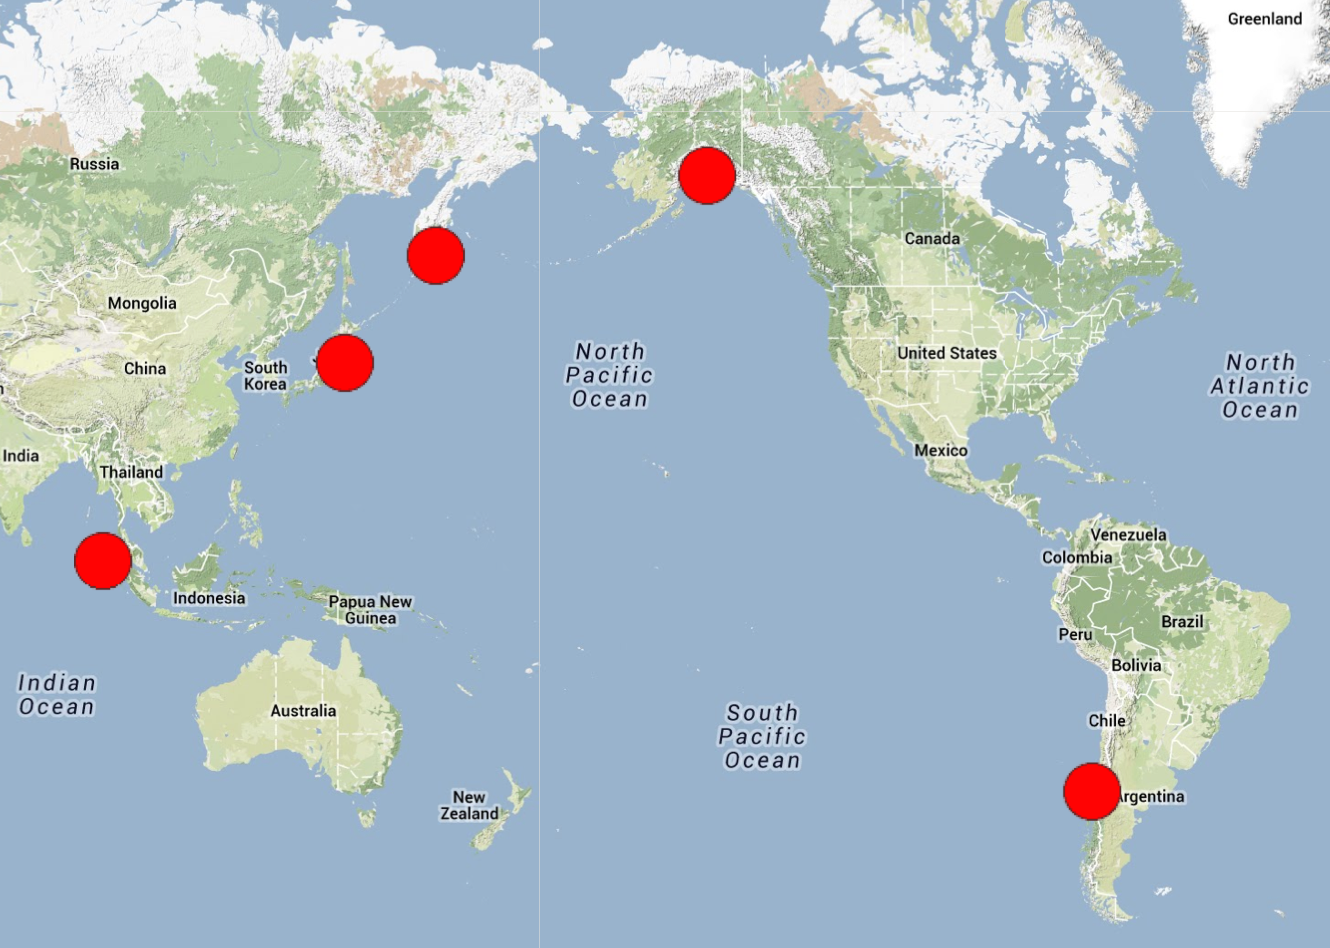
\includegraphics[width=0.50\textwidth]{M9}
   \caption[Sismos com magnitude acima de 9,0.]
   		   {Sismos com magnitude acima de 9,0.} 
   \label{f:m9}
\end{figure} 


Tremores de terra, abalos, \glspl{equake}, sismos são a ocorrência de
fenômenos geológicos de ruptura, instantânea, por certo mecanismo, de certa dimensão, na
crosta terrestre.

\subsection{Ocorrência}
\index{\gls{equake}!ocorrência}
\label{sec:ocorrencia}
 
Os tremores acontecem por uma ruptura geológica (figura \ref{f:rupture}) num tempo \gls{sym:t}, num lugar \gls{sym:r} e cada um
com seu tamanho \gls{sym:m}.

\begin{figure}[H]
   \centering
   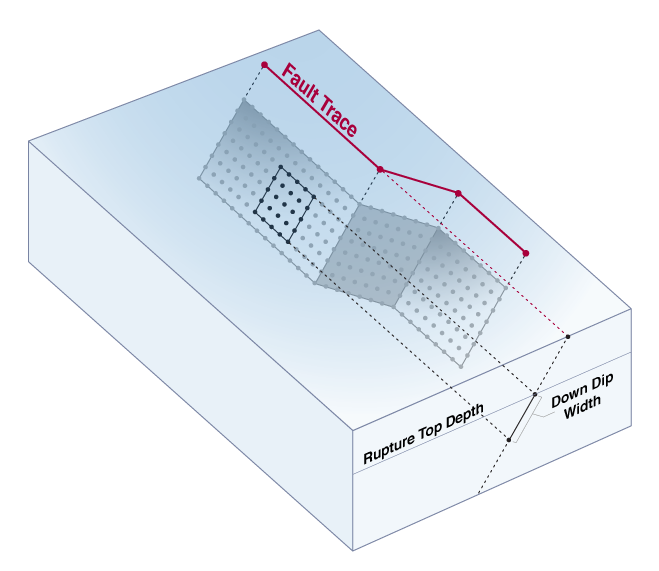
\includegraphics[width=0.50\textwidth]{rupture}
   \caption[Ilustração da área de ruptura em um falhamento geológico]
   		   {Ilustração da área de ruptura em um falhamento geológico\footnotemark} 
   \label{f:rupture}
\end{figure} 
\footnotetext{\citet{img_opensha_rupture}}
 

O local em que se iniciou a ruptura que deu origem ao tremor é um \gls{hypocenter},
enquanto sua projeção na superfície, desconsiderando-se a profundidade, é o \gls{epicenter}.


\subsection{Magnitude (da ruptura)}
\index{magnitude}
\label{sec:magnitude}

A magnitude de um tremor de terra é um valor medido numa escala que versa sobre a energia liberada pelo sismo, que é 
proporcional a área rompida e ao deslocamento geológico relativo entre as partes rompidas.

O desenvolvimento experimental de escalas de magnitude, para medir o tamanho dos tremores,
é marcado pelo trabalho do sismólogo Charges Richter \citep{richter_1935}.

Existem, entretanto, uma série de diferentes escalas de magnitude,
baseadas em diversos tipos de medidas. 

A escolha de qual usar fica a critério
de cada operador de sismógrafo e de cada rede sismográfica, que geralmente usam escalas diferentes
para avaliar a magnitude dos tremos, ou até mesmo divulgam mais de um tipo para
um mesmo evento.

As escalas são calibradas para fornecerem valores similares, de acordo com
o intervalo de utilidade para o qual foram desenvolvidas, mas apresentam diferenças consideráveis para um mesmo evento, 
podendo comprometer as análises estatísticas baseadas num catálogo cuja magnitude não tenha sido calculada de maneira uniforme.


\subsubsection{Magnitude Richter}
\index{magnitude!Richter}
\label{sec:magnitude_richter}

As escalas de magnitude mais comuns são as que derivam da definição de Richter \citep{richter_1935}
que se baseia na relação empírica entre o logarítmo da amplitude do registro das ondas sísmicas e a distância onde foram
registradas. Em 1935, Richter notou que:

\begin{equation}
	\gls{eqn:richter}
	\label{eq:richter}
\end{equation}
\glsdesc*{eqn:richter}.


A amplitude máxima de sua
escala foi definida pela amplitude máxima observada em um sismômetro Wood-Anderson, com período de 0.8s, registrando a 100km 
do tremor.

Na prática existem algumas incertezas e correções que deveriam ser feitas, principalmente pelo fato da escala estar intimamente 
relacionada a um determinado equipamento, hoje obsoleto, e porque que sismos locais (a menos de 100km) têm sua magnitude
melhor calculada usando frequencias mais altas que as registráveis pelo sismômetro da época.


Outras escalas foram desenvolvidas a partir da medida da amplitude máxima de determinadas fases 
(diferentes tipos de onda sísmica) e apresentam bons resultados para a maior parte dos sismos.
Não refletem, porém, com precisão, o tamanho dos maiores e mais destrutivos eventos, com magnitude acima de 7 ou 8.


\subsubsection{Magnitude de Momento Sísmico }
\index{magnitude!momento sísmico}
\label{sec:risco_sismico}

O evento de natureza sismológica ocorre num
instante \gls{sym:t} liberando uma certa quantidade de energia na forma de \glsdesc{sym:M_0}
\gls{sym:M_0} proporcional à \glsdesc{sym:M_W} \gls{sym:M_W} desse evento.

O \glsdesc{sym:M_0} é apresentado na equação \ref{eq:M_0}:

\begin{equation}
	\gls{eqn:M_0}
	\label{eq:M_0}
\end{equation}
\glsdesc*{eqn:M_0}.

O momento sísmico é estimado geralmente pela inversão duplamente acoplada de um tensor de momento aos registros em 
forma de onda do movimento do chão causado pelo terremoto. Ou, em casos de tremores muito bem registrados, ele pode
ser estimado a partir de algum modelo numérico para a ruptura.

A \glsdesc{sym:M_W} \gls{sym:M_W} \citep{hanks_1999} é baseada no 
logarítmo do \glsdesc{sym:M_0} \gls{sym:M_0}, e não se satura no caso de grandes eventos. 
Sua definição é dada pela equação \ref{eq:M_W} 

\begin{equation}
	\gls{eqn:M_W}
	\label{eq:M_W}
\end{equation}
\glsdesc*{eqn:M_W}.


\subsubsection{Intensidade Macrossísmica}
\index{instensidade macrossísmica}
\label{sec:intensidade}

A intensidade macrossísmica é uma escala para medir, não a energia proporcional
à ruptura que originou o tremor de terra, mas para retratar a percepção humana do
movimento do chão onde quer este tenha produzido seus efeitos.

Uma das mais difundidas é a escala Modificada de Mercalli \citep{richter_1958} apresentada em sua versão simplificada 
na tabela \ref{tab:mercalli}:

\begin{table}[H]
\begin{center}
\begin{scriptsize}
\noindent\begin{tabular}{c|c|p{12cm}}
\hline
Categoria  	& Sensação & Efeitos \\
\hline
I 			&	Imperceptível 	&	Não sentido. Apenas registado pelos sismógrafos.
\\II 		&	Muito fraco 	&	Sentido por um muito reduzido número de pessoas em 
								repouso, em especial pelas que habitam em andares
								elevados.
\\III 		&	Fraco 			&	Sentido por um pequeno número de pessoas. Bem sentido nos andares elevados.
\\IV 		&	Moderado 		&	Sentido dentro das habitações, podendo despertar do sono um pequeno número de pessoas. 
								Nota-se a vibração de
								portas e janelas e das loiças dentro dos armários.
\\V 		&	Forte 			&	Praticamente sentido por toda a população, fazendo acordar muita gente. 
								Há queda de alguns objectos menos estáveis e param os pêndulos dos relógios. 
								Abrem-se pequenas fendas nos estuques das paredes.
\\VI 		&	Bastante forte 	&	Provoca início de pânico nas populações. Produzem-se leves danos nas habitações, 
								caindo algumas chaminés. O mobiliário menos pesado é deslocado.
\\VII 		&	Muito forte 	&	Caem muitas chaminés. Há estragos limitados em edifícios de boa construção, 
								mas importantes e generalizados nas construções mais frágeis. 
								Facilmente perceptível pelos condutores de veículos automóveis em trânsito. 
								Desencadeia pânico geral nas populações.
\\VIII 		&	Ruinoso  		&	Danos acentuados em construções sólidas. Os edifícios de muito boa construção 
								sofrem alguns danos. Caem campanários e chaminés de fábricas.
\\IX 		&	Desastroso 		&	Desmoronamento de alguns edifícios. Há danos consideráveis em construções muito sólidas.
\\X 		&	Destruidor 		&	Abrem-se fendas no solo. Há cortes nas canalizações, torção nas vias de caminho 
								de ferro e empolamentos e fissuração nas estradas.
\\XI 		&	Catastrófico 	&	Destruição da quase totalidade dos edifícios, mesmo os mais sólidos. 
								Caem pontes, diques e barragens. Destruição das redes de canalização e das vias de comunicação. 
								Formam-se grandes fendas no terreno, acompanhadas de desligamento. Há grandes escorregamentos de terrenos.
\\XII 		&	Cataclismo 		&	Destruição total. Modificação da topografia. Nunca foi presenciado no período histórico. \\
\hline
\end{tabular}
\caption{Escala simplificada de intensidade sísmica, modificada em 1956 a partir da escala original de Giuseppe Mercalli de 1902}
\label{tab:mercalli}
\end{scriptsize}
\end{center}
\end{table}

Existem estudos \citep{bakun_1999} que propõem a inferência sobre o tamanho da ruptura, e sua
magnitude, a partir de observações macrossísmicas, ou dos efeitos relatados pela escala de intenside, georreferenciados.


%% ------------------------------------------------------------------------- %%
\subsection{Catálogos}
\index{catálogos}
\label{sec:catalogos}

Os catálogos podem ser vistos como uma coleção de parâmetros sobre os tremores. 
Podem ser classificados em três categorias \citep{woessner_catalog_2010} enumeradas a seguir:

\begin{itemize}\setlength{\itemsep}{0em}
	\item Pré-históricos: baseados na coleta de dados feitas por 
	geólogos estruturais em trincheiras ou campos de subsidência. Podem conter registros de tremores que ocorreram 
	há milhares de anos.
	\item Históricos: catálogos formados a partir de relatos históricos e inferência de valores de intensidade
	(seção \ref{sec:intensidade}), de análises de forma de onda com instrumentos antigos (registros em papel), eventualmente
	digitalizados.
	Cobrem o período das primeiras descrições humanas até os catálogos intrumentais.
	\item Instrumentais: são os catálogos de sismicidade definidos por dados produzidos por uma rede sismográfica bem estabelecida
	 gerando localizações continuamente (que começam a existir a partir de 1970).
\end{itemize} 

Os catálogos instrumentais são uma listagem onde se epera que encontrar para cada evento as seguintes informações:

\begin{itemize}\setlength{\itemsep}{0em}
	\item algum identificador,
	\item a localização (\gls{hypocenter}) do evento em algum sistema de referência (longitude, latitude, profundidade),
	\item o tempo de origem: data e hora com precisao de pelo menos décimos de segundo e
	\item uma ou várias informações de \glsdesc{sym:m}.
\end{itemize} 

Adicionalmente, embora não seja muito frequente, podem ser fornecidas informações adicionais obtidas pela análise das formas de
onda, como:

\begin{itemize}\setlength{\itemsep}{0em}
	\item incertezas sobre as magnitudes,
	\item incertezas sobre a localização (erro padrão, elipses de erro, cobertura dos sismogramas em diversas distâncias, cobertura
	dos sismogramas em vários ângulos azimutais, acurácia do modelo de velocidades utilizado, para enumerar alguns),
	\item intensidade máxima,
	\item intensidade no epicentro,
	\item número de, e as vezes as próprias, informações usadas para a determinação do hipocentro e hora de origem,
	\item sobre o mecanismo (alinhamento, mergulho e sentido do deslocamento na falha geológica) focal, entre outras.
\end{itemize} 

Mas é importante salientar \citep{woessner_catalog_2010} que cada um dos parâmetros determinados é fruto de uma série de decisões
e etapas de processamento.

Começam pela escolha dos sismômetros a serem instalados e onde para registrar as formas de onda. Sinais acima do nível de ruído
são associados à chegadas de fases quando registradas em mais de uma estação. 

A localização e o tempo de origem são
determinados juntando-se os tempos de chegadas das fases a um modelo de velocidade das ondas ao longo de camadas da crosta (ao
qual a localização é extremamente dependente). 

As magnitudes são computadas a partir das amplitudes e/ou da duração do sinal, dependendo profundamente da calibração dos
instrumentos.

\subsection{\glsdesc{mfd}}
\index{MFD}
\label{sec:mfd}

Observa-se que os sismos menores são muito mais frequêntes.
Entretanto, os maiores e mais raros são os que trazem a maior ameaça e os que causam as maiores perdas.

Uma análise conveniente seria explorar como se dá essa distribuição de magnitudes.

\subsubsection{\gls{mfd} de Gutenberg-Richter}
\index{Gutenberg-Richter MFD}
\label{sec:grmfd}

Gutenberg e Richter \citep{gr_1954} observaram empiricamente que a distribuição da frequência de ocorrência dos tremores e das
magnitudes seguiam uma deistribuição cuja versão clássica é apresentada na equação \ref{eq:gr_mfd} a seguir:

\begin{equation}
	\gls{eqn:gr_mfd}
	\label{eq:gr_mfd}
\end{equation}
\glsdesc*{eqn:gr_mfd}.

Com uma simples transformação de variáveis ($\alpha = 10^a$ e $\beta = b\ln{10}$), observa-se que o número de sismos que ocorrem 
com magnitudes dentro de um pequeno intervalo $[m, m+dm]$ tem distribuição exponencial:

\begin{equation}
	\begin{split}
		\gls{sym:N_m} &= 10^{\gls{sym:a} - \gls{sym:b}\gls{sym:m}} \\
					  &= \alpha e^{-\beta m}
	\end{split}
	\label{eq:gr_exp}
\end{equation}

A distribuição cumulativa, ou seja, o número de eventos com magnitude maior que um certo valor $m_{min}$ também segue uma
distribuição exponencial e é apresentada na equação \ref{eq:gr_cum}:

\begin{equation}
	\begin{split}
		N(m > m_{min}) &= \alpha \int\limits_{m_{min}}^{\infty}e^{-\beta m}\mathrm{d}m \\
					   &= \frac{\alpha}{\beta} e^{-\beta m} \\
					   &= \alpha_{cum} e^{-\beta m}
	\end{split}
	\label{eq:gr_cum}
\end{equation}
onde $\alpha_{cum} = \alpha / \beta $ é o valor cumulativo da atividade sísmica.


Entretanto, a distribuição clássica de \gls{gr} não impunha restrições sobre um limite inferior $m_{min}$ 
ou superior $m_{max}$ à validade da distribuição.



\subsubsection{MFD Truncada}
\index{MFD Truncada}
\label{sec:TMFD}

Variações da distribuição clássica de \gls{gr} foram propostas em vista de melhor representar as MFD estudadas à partir de
catálogos de diversas regiões.

A equação \ref{eq:gr_max} versão incremental truncada com um limite superior $m_{max}$:

\begin{equation}
		\gls*{sym:N_m} = \frac{e^{-\beta m}}{1 -e^{-\beta m_{max}} }, m \leq m_{max}
	\label{eq:gr_max}
\end{equation}

Na equação \ref{eq:gr_dtr} versão incremental duplamente truncada com um limite inferior $m_{min}$ e superior $m_{max}$ :

\begin{equation}
		\gls*{sym:N_m} = \frac{e^{-\beta (m - m_{min})}}{1 -e^{-\beta (m_{max} - m_{min}) } } , m_{min} \leq m \leq m_{max}
	\label{eq:gr_dtr}
\end{equation}

A figura \ref{f:mfd} ilustra essas distribuições.

\subsubsection{MFD Limitada}
\index{MFD Limitada}
\label{sec:BMFD}

Outra possibilidade, é limitar suavemente a parte final da curva (ver figura \ref{f:mfd}). A equação \ref{eq:gr_bounded} apresenta
a distribuição:

\begin{equation}
		\gls*{sym:N_m} = \alpha [ e^{-\beta (m - m_{min})} - e^{-\beta (m_{max} - m_{min}) } ], m_{min} \leq m \leq m_{max}
	\label{eq:gr_bounded}
\end{equation}


\subsubsection{MFD com decaimento exponencial}
\index{MFD com decaimento exponencial}
\label{sec:KMFD}

Yan Kagan \citep{kagan_2002} propôs uma distribuição de magnitude mais adequada e acoplada à energia liberada pelos sismos, que
pode ser descrita como na equação \ref{eq:gr_tapered}:

\begin{equation}\ensuremath{
		\gls*{sym:N_m} = [\gls*{sym:beta_p} + \frac{m}{m_{min}}]
				m_{min}^{\gls*{sym:beta_p}}
				\gls*{sym:m_corner}^{-1 -\gls*{sym:beta_p}}
				e^{\frac{m_{min} - m}{\gls*{sym:m_corner}}}, 
				m_{min} \leq m < \infty
		}
	\label{eq:gr_tapered}
\end{equation}
onde \glsdesc*{sym:beta_p} e \gls*{sym:m_corner} \glsdesc*{sym:m_corner}

A figura \ref{f:mfd} mostra a diferença entre algumas dessas distribuições

\begin{figure}[H]
   \centering
   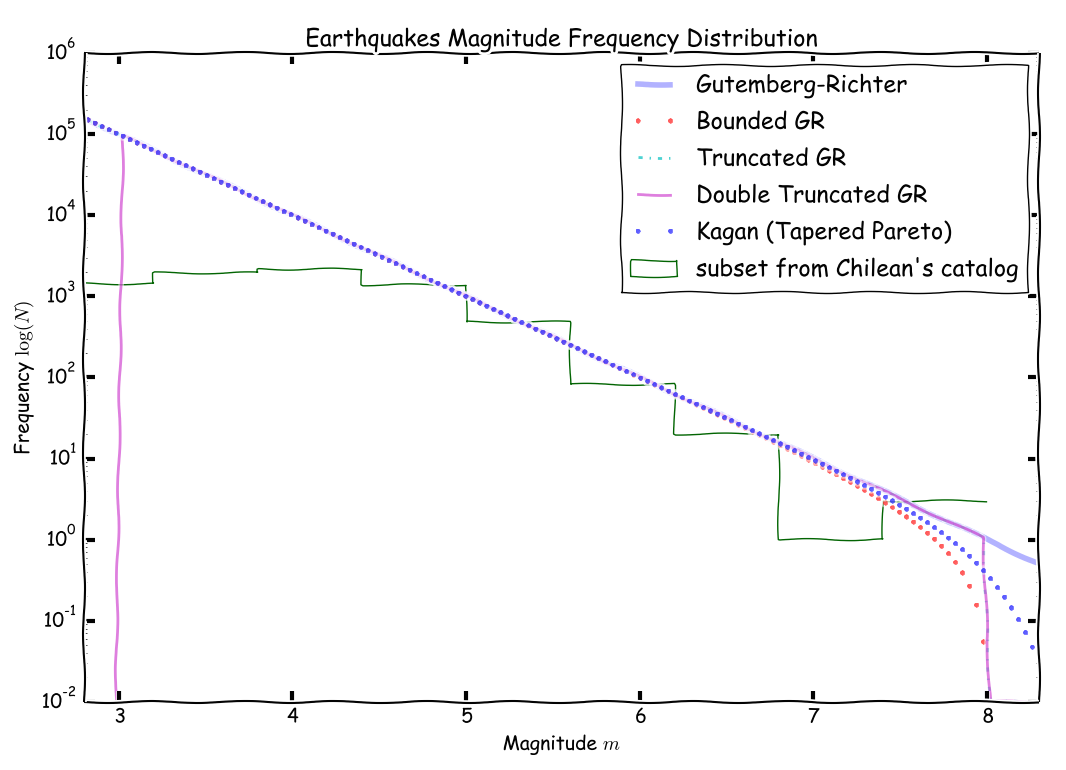
\includegraphics[width=0.95\textwidth]{mfd}
   \caption[Distribuições de frequência e magnitude]
   		   {Distribuições de frequência e magnitude} 
   \label{f:mfd}
\end{figure} 

A figura \ref{f:mfd} apresenta um comparativo de algumas distribuições. Para ilustração, há também um histograma de um catálogo de
uma pequena região do norte do Chile, onde se pode observar que tanto a porção inferior (em torno de $m=5$), como a porção
posterior ($m > 7$) do histograma não seguem perfeitamente a distribuição. Há essencialmente duas zonas críticas em que é preciso
estar atento à física do problema:
(i) na parte inferior, muitos sismos de magnitude pequena não são registrados, seja por não terem energia suficiente
para sensibilizar um conjunto razoável de estações que permitam determinar suas localizações, seja porque o número de
estações é insuficiente na região onde os pequenos tremores ocorrem; (ii) a parte superior, por sua vez, é crítica
por se acoplar diretamente aos limites físicos do tamanho da maior ruptura possível, relacionada diretamente ao limite de liberação de energia na forma de momento sísmico $M_0$.

Nas distribuições de magnitude e frequência é importante que se possa reconhecer claramente alguns parâmetros
fundamentais.

\subsection{Valor-b}
\index{valor-b}
\label{sec:b_value}

O \emph{valor-b} foi apresentado nesta seção como a inclinação da reta que representa a parte plana descrescente da
distribuição. Representa a proporção de sismos pequenos e catastróficos que uma determinada fonte sísmica é capaz de
produzir.


\begin{figure}[H]
   \centering
   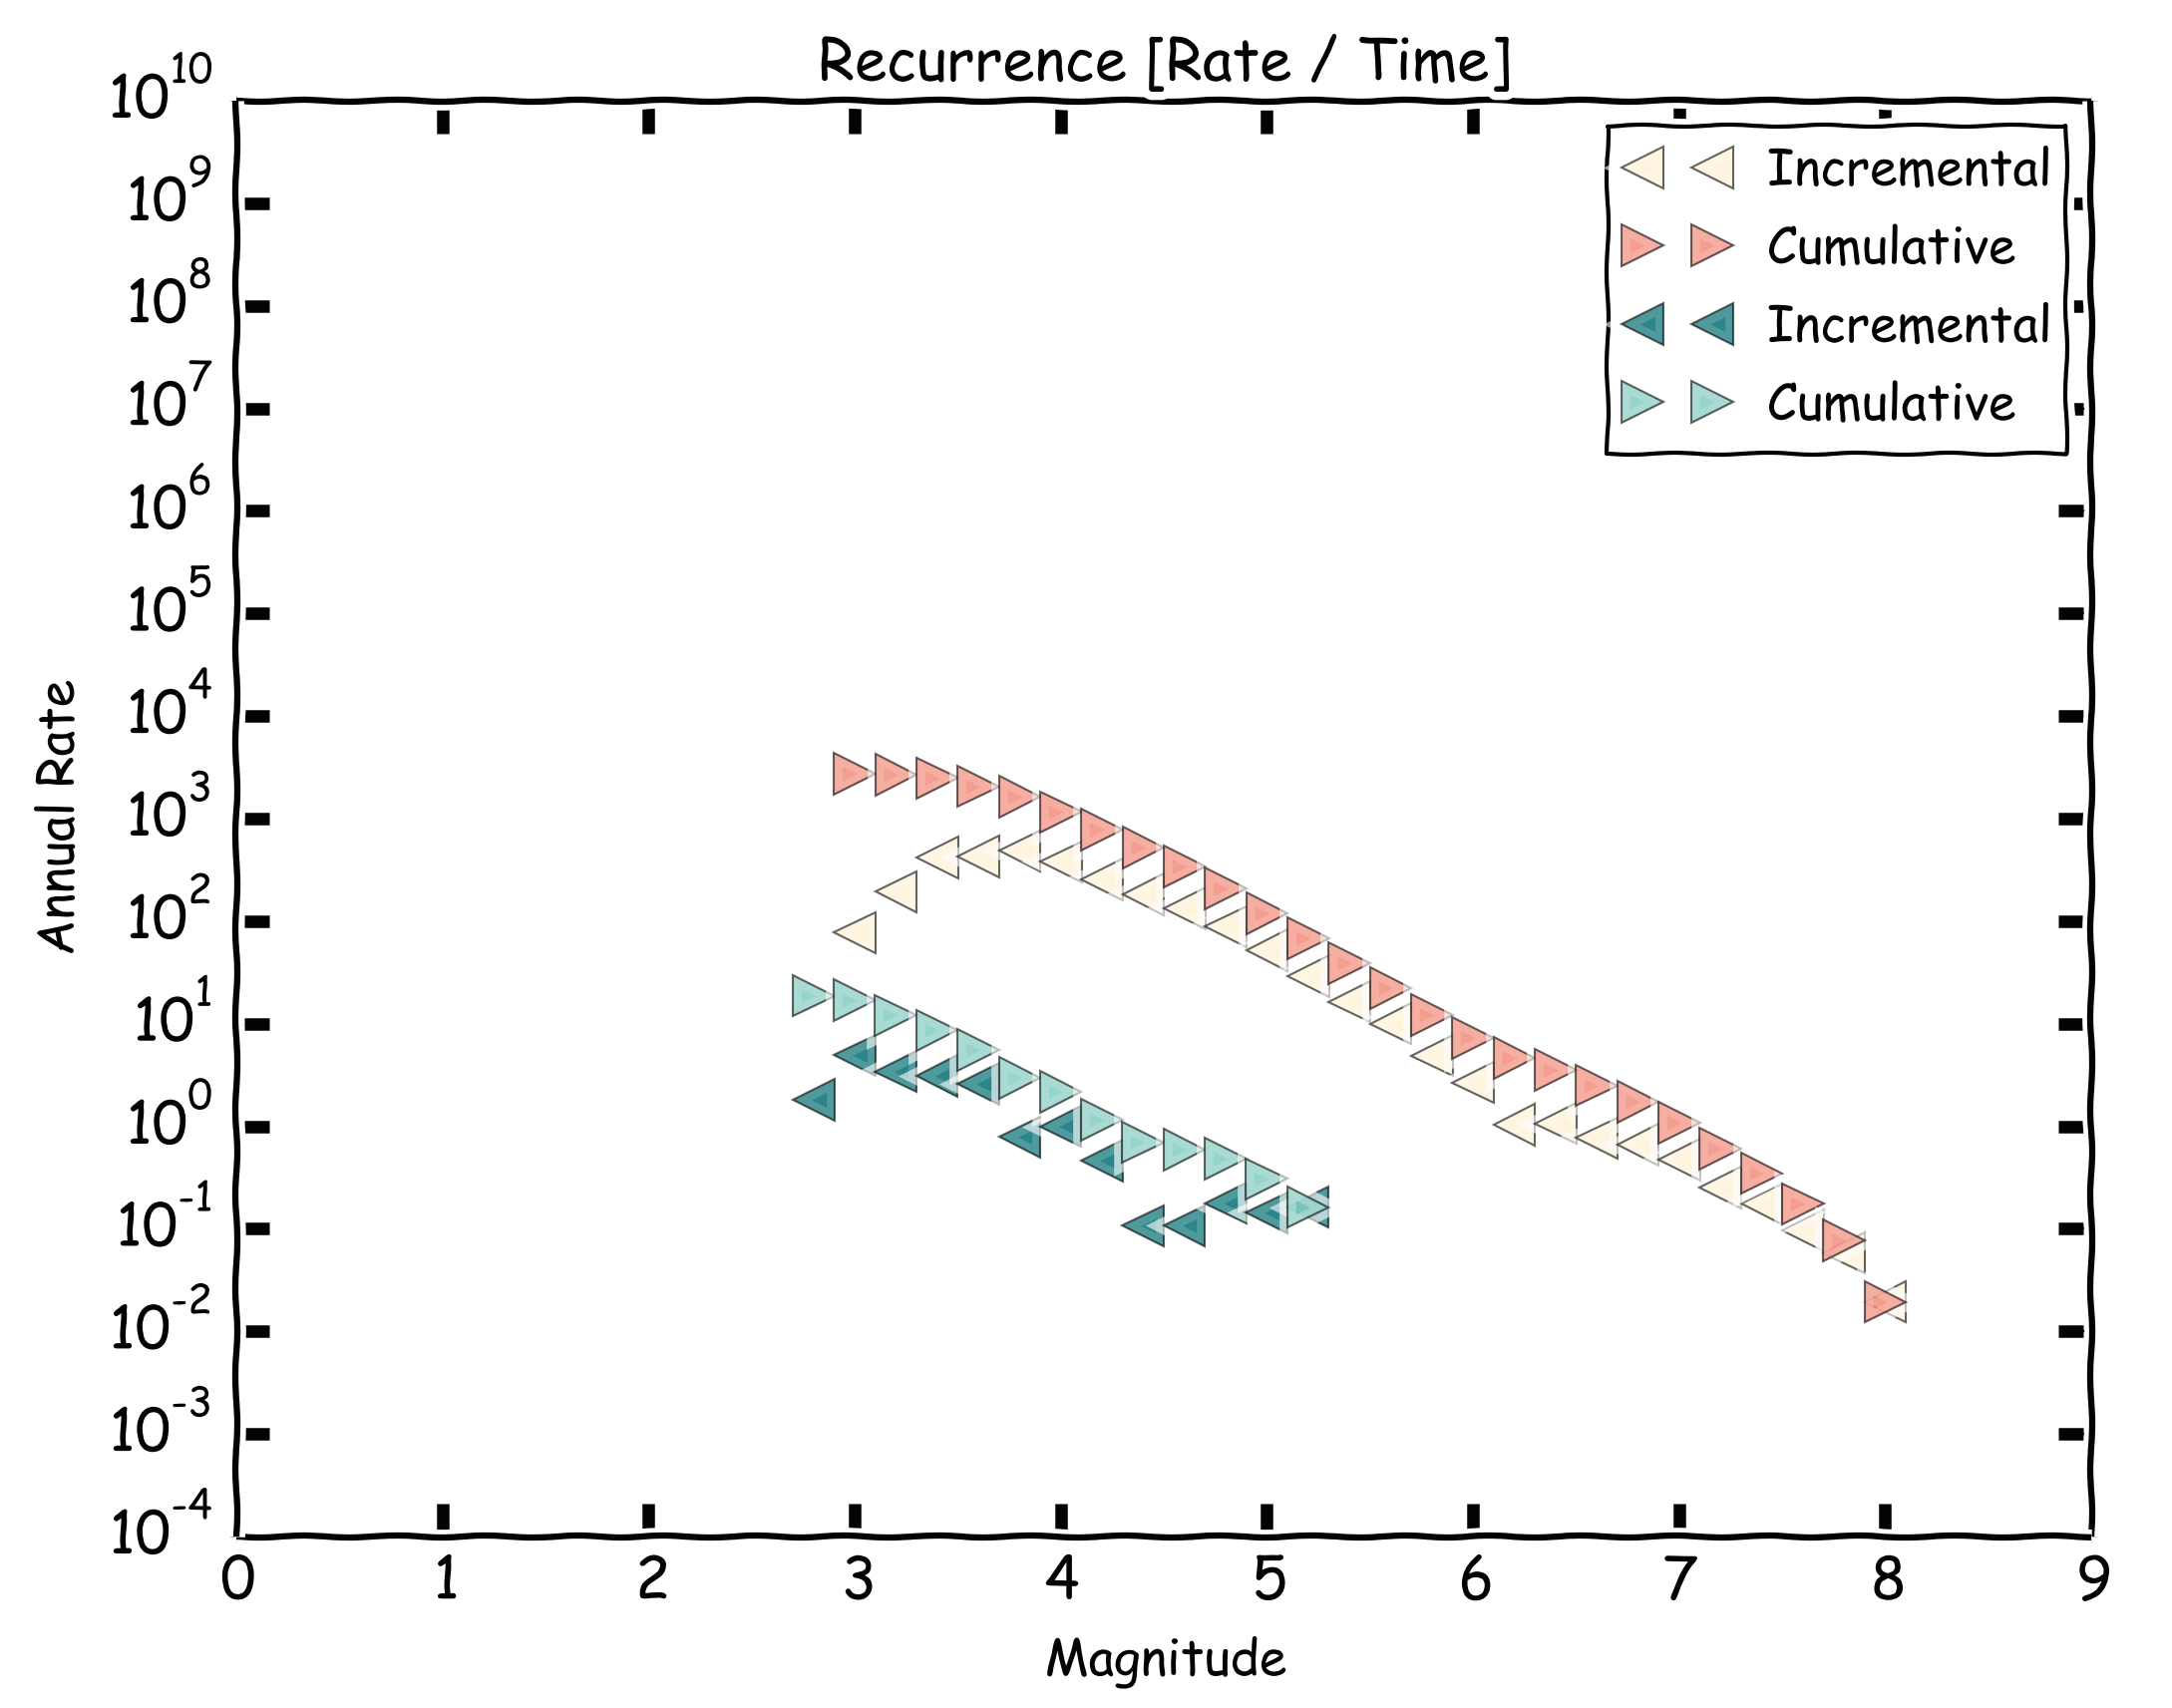
\includegraphics[width=0.50\textwidth]{occurrence}
   \caption[Distribuição incremental e cumulativa de frequencia e magnitude dos sismos presentes no catálogo ISC-GEM
   para a América do Sul unido com o BSB2013]
   {Distribuição incremental e cumulativa de frequencia e magnitude dos sismos presentes no catálogo ISC-GEM
   para a América do Sul unido com o BSB2013} 
   \label{f:occurrence}
\end{figure} 
%\footnotetext{\citet{img_opensha_rupture}}
 




\subsection{Taxa de Sismicidade}
\index{taxa de sismicidade}
\label{sec:seismic_rate}

A taxa de sismicidade é a medida da ocorrência dos tremores por uma determinada unidade de tempo (geralmente anos).
Representa para cada magnitude, a frequência média de ocorrência (\gls{sym:lambda} do processo de Poisson).

\subsection{Valor-a}
\index{valor-a}
\label{sec:a_value}

O \emph{valor-a} é a projeção da \gls{mfd} no eixo das frequências e representa o nível geral de sismos
que as fontes observadas pelo catálogo são capazes de produzir.

Costuma ser confundido pela forma de representação adotadas para a distribuição (incremental e/ou
cumulativa) e pelos truncamentos onde por vezes se apresenta o valor-a como a taxa de sismicidade da 
magnitude mínima ou de completude do catálogo.

No presente trabalho o valor-a significará sempre o valor-a da distribuição cumulativa de sismos por unidade de tempo
com magnitudes positivas.

\subsection{Magnitude de Completude}
\index{magnitude de completude}
\label{sec:completeness}

A magnitude de completude é o valor mínimo para o qual a distribuição é capaz de observar o conjunto completo dos
sismos. Em outras palavras representa o limite de observação completa do catálogo.

Sua identificação é bem simples quando se observa a distribuição incremental de magnitudes. É facilmente notado o valor
de magnitude na porção inferior na qual o número de sísmos registrados começa a divergir da tendência geral da
distribuição.

Seu mapeamento é importante uma vez que os métodos de ajuste e determinação dos parâmetros da distribuição baseados na
máxima verossimilhança (REFERENCIA) dependem fundamentalmente desse valor mínimo.



FIGURA SouthAm ISC-GEM



\section{Risco Sísmico}
\index{Risco Sísmico}
\label{sec:risco_sismico}

A redução do risco sísmico é um problema complexo que envolve geralmente muitas pessoas, informações, decisões e ações.

A palavra risco, ao pé da letra, significa a exposição à possibilidade de injúria ou perda. E geralmente é usada como
sinônimo de ameaça. Na literatura acerca do tema risco, inclusive, as palavras risco e ameaça são usadas com certa
confusão.

No glossário da EERI (EERI Committee on Seismic Risk, 1984) a definição de risco sísmico é a probabilidade de que
perdas sociais ou econômicas aconteçam como decorrência de tremores por superarem limiares estabelecidos para
determinado local ou região durante um certo período de exposição.

A ameaça sísmica, por outro lado, é qualquer fenômeno físico (oscilação, falhamento) associado à terremotos que possam
produzir efeitos adversos às atividades humanas. Na prática são avaliados por dadas probabilidades de ocorrência.

Do que se pode deduzir que o risco sísmico é uma combinação da ameaça sísmica com outros fatores:

\begin{equation}
		Seismic Risk = Seismic Hazard \ast Vulnerability \ast Exposed Value
	\label{eq:risk}
\end{equation}

onde a vulnerabilidade é a quantidade de danos induzidos por um dado grau de ameaça e expressa como uma fração do
valor exposto ao dano e varia de acordo com o modelo proposto.

Frequentemente, o fator vulnerabilidade advém das análises das (ii) respostas das estruturas edificadas ao espectro de
acelerações produzidos pela (i) provável ameaça sísmica e da análise de possíveis (iii) danos estruturais à edificação.

A decisão de alterar ou não o desenho estrutural das edificações é feito a partir da análise dos (iv) prejuízos
(quantidade de moeda, mortes, tempo inoperante) causados caso as estruturas sejam danificadas conforme as análises anteriores.


\section{Ameaça Sísmica}
\index{ameaça sísmica}
\label{sec:ameaca_sismica}

A ameaça sísmica poderia ser definida de mode geral como a possibilidade de ocorrer efeitos potencialmente destrutivos
de um terremoto em uma particular localização. Com exceção de \textit{tsunamis} ou falhamentos geológicos superficiais,
todos os efeitos destrutivos de um tremor de terra estão diretamente relacionados ao movimento do chão induzido pela
passagem das ondas sísmicas. Existem, entretanto diferenças de abordagem para a avaliação da ameaça sísmica.

A \gls{psha} foi introduzida por Cornell (1968) e se tornou técnica mais amplamente usada para a avaliação da
ameaça sísmica, mas também se pode fazer a avaliação através de cenários determinísticos definidos pelo espectro de
movimento forte do chão que pode ser caudado pela ocorrÊncia de um determinado tremor de terra em certa localização e
de certa magnitude. O possível movimento forte no local de interesse é avaliado através de relações de atenuação ou
\gls{gmpe}.

Os mecanismos da \gls{psha} são menos óbvios do que os da \gls{dsha} e em essência significam identificar todos os
possíveis tremores que podem afetar o local de interesse, incluíndo todas as possíveis combinações de distâncias e
caracterizar a frequência de ocorrência das diferentes magnitudes através de relações de recorrência. As equações de
atenuação são utilizadas para calcular os parâmetros do movimento do chão no local de interesse devido a esses tremores
e consequentemente a taxa com que diferentes níveis de movimento do chão ocorram no local de interesse. 

Seus resultados também apresentam certa distinção. Se por um lado a \gls{psha} traz consigo o aspecto temporal, ou a
taxa com que diferentes níveis de aceleração excederão determinado limiar em determinado local de interesse,
por outro, a \gls{dsha} apresenta o movimento do chão esperado quando ocorra determinado evento de controle.

TODO:
(Cornell, 1968) 
DSHA  (Reiter, 1990; Kramer,1996; Krinitzsky, 2002)

(Cornell, 1968;  Bazzurro and Cornell, 1999; Abrahamson, 2000b; Hanks and Cornell, 2001; Abrahamson, 2006) 

differences bommer, 1998
 
\subsection{Projeção da Ocorrência de Rupturas}
\index{projeção de ocorrência de rupturas}
\label{sec:projecao}

As projeções (\textit{forecasting}) são feitas para se estimar a ocorrência de futuros tremores,
principalmente dos maiores, com grandes chances de provocar perdas.

Nas de curto prazo, estimam-se os próximos tremores
numa escala de dias ou horas considerando uma taxa de sismicidade variável 
com o tempo como no caso dos pré e pós-abalos, ou de quando 
acontece um enxame sísmico, período de maior atividade numa região.
Sua principal aplicação é a auxiliar na tomada de decisões de curto período, 
como evacuação de edifícios.

Nas de longo prazo, foco desse texto, a principal consideração feita é de que a 
\gls{seismic_rate} não varie ao longo do tempo, servindo para estimar as acelerações 
provovadas por tremores que possam ocorrer,
mesmo que muito raramente, de grandes proporções. Suas aplicações fazem sentido quando
se deseja saber o nível de segurança e resistência estrutural que devem ser impostos 
às edificações em geral, ou o valor de um contrato de resseguro de plataformas de petroleo,
ou outros grandes investimentos industriais, como usinas nucleares.


\section{Análise Probabilística de Ameaça Sísmica}
\index{PSHA, Análise Probabilística de Ameaça Sísmica}
\label{sec:psha}

Na \gls{psha} são considerados todos os possíveis tremores, as rupturas que os originaram e os movimentos do chão
resultantes conjuntamente com suas probabilidades de ocorrência associadas de modo a encontrar o nível de movimento do
chão que será excedido com uma determinada baixa tolerância (BAKER)

Se por um lado Cornell foi um dos pioneiros em desenvolver e apresentar a medotologia da \gls{psha}, McGuire (1976)
introduziu importantes elementos com seu software EQRISK. Mas fundamentalmente o método consiste de dois pilares, o
primeiro é a definição de zonas sismogênicas como áreas ou linhas em cuja sismicidade deveria ser considerada
espacialmente uniforme. O segundo é o pressuposto de que a sismicidade pode ser representada por um processo de Poisson.
Os dois têm sido de uma maneira ou outra questionados e pesquisadores ainda propõem alternativas.

Uma \gls{psha} pode ser separada em cinco passos para uma melhor compreensão:

\begin{itemize}
\item Identificar todas as fontes sísmicas capazes de produzir movimentos do chão potencialmente danosos.
\item Caracterizar a distribuição de magnitudes (taxa de esperada de ocorrência para cada magnitude possível de tremor).
\item Caracterizar a distribuição de distâncias dos tremores ao local de interesse associada com cada potencial fonte
sísmica.
\item Prever a distribuição resultante da intensidade do movimento do chão devido à distância do tremor, à
magnitude, à condições geológicas do local de interesse, etc.
\item Combinar as incertezas dos prováveis locais de origem, das prováveis magnitudes e dos prováveis movimentos
do chão causados pelos tremores de terra usando o teorema da probabilidade total.
\end{itemize}

Os diferentes métodos de \gls{psha} variam propondo alterações em uma ou mais de uma dessas etapas detalhadas a seguir.

%% ------------------------------------------------------------------------- %%
\subsection{Identificação das fontes sísmicas}
\index{\gls{psha}!identificação das fontes}
\label{sec:psha_sources}


Para identificar fontes sísmicas são utilizados desde registros históricos de sismicidade à evidências geológicas de
falhamentos/rupturas datados com deslocamento e magnitudes inferidos e busca-se aproveitar de toda informação relevante
disponível, como a medida secular de deslocamento relativo entre observaçõe geodésicas contínuas ou mesmo da sismicidade recente.


\subsubsection{Tipologia e Representação Geométrica}
\index{Tipologia e Representação Geométrica}
\label{sec:fontes_tipologia}

Quando se identifica uma fonte sísmica é comum representá-la segundo uma forma geométrica mais consistente com o
conjunto das observações disponíveis para descrever as possíveis rupturas.

\subsubsection{Ponto}
\index{fonte sísmica!ponto}
\label{sec:point_source}

Se apenas se conhece a localização isolada de um tremor antigo, com magnitude e com mecanismo de falhamento conhecido,
é possível representá-lo como uma fonte sísmica de tipo pontual. Nesse tipo de fonte são definidos os limites superior e
inferior da ruptura, sua orientação e tipo de falhamento (quando disponíveis) e o hipocentro é definido a partir do
centro de cada ruptura.

\subsubsection{Área}
\index{fonte sísmica!área}
\label{sec:area_source}

Quando o conhecimento sobre a geologia, a tectônica, ou mesmo a correlação espacial dos tremores no catálogo, permitam
o delineamento de zonas com características sísmicas comuns, se costuma representar como áreas com forma poligonal onde
por fim serão discretizadas como um conjunto de fontes sísmicas de característica pontual distribuída uniformemente por
toda área.

\subsubsection{Falha Simples}
\index{fonte sísmica!falha simples}
\label{sec:simple_fault_source}

Muitas vezes os parâmentros de um falhamento ativo são claramente conhecidos e monitorados. Isso permite uma maior
especificidade na representação da fonte sísmica, diminuindo, por exemplo, as incertezas na orientação das rupturas.
Nesse caso a geometria da falha se caracteriza pela projeção do traço de falha na superfície e pelos limites superior e
inferior da ruptura no plano de mergulho.


\subsubsection{Falha Complexa}
\index{fonte sísmica!falha complexa}
\label{sec:complex_fault_source}

Casos de sismicidade mais complexa como zonas de subdução ou encontro de placas, tem uma sismicidade mais complexa,
gerada por estruturas maiores e mais proundas que apresentam geralmente variações laterais de mergulho, acúmulo de
esforços, orientação, etc. Fontes sísmicas em situações como essa são modeladas por como múltiplos segmentos simples e
unidos de forma suave.


\subsection{Caracterização da \gls{mfd}}
\index{caracterização da \gls{mfd}}
\label{sec:psha_mfd}

Conhecida a fonte sísmica e sua representação geométrica, é preciso caracterizar sua capacidade sismogênica determinando
uma (ou mais) possíveis \gls{mfd} a que se ajustam as observações. Isso inclui a forma da distribuição, a taxa geral de
sismicidade (valor-a) e frequentemente as magnitudes mínima e máxima. 

\subsection{Caracterização da Distribuição de Distâncias}
\index{caracterização da distribuição de distâncias}
\label{sec:psha_distances}

Dados um local de interesse e uma provável ruptura em uma fonte sísmica, é necessário calcular a distribuição das
distâncias da fonte ao local de interesse.

É necessário calcular a distribuição da distância das possíveis rupturas em uma fonte sísmica à um determinado local de
interesse.


\subsection{Predição do Movimento do Chão}
\index{predição do movimento do chão}
\label{sec:gmpe}

Para se estimar os possíveis níveis de movimento do chão causados por eventos de uma determinada magnitude à uma certa
distância do local de interesse são utilizadas as \glspl{gmpe}.

forma geral da gmpe

Exemplo de modelagem de gmpe


\subsection{Combinação de Incertezas e Avaliação da Ameaça Sísmica}
\index{cálculo da ameaça}
\label{sec:hazard}


Integral do Hazard\ldots.

